\documentclass[10pt, compress, xcolor={table,xcdraw,usenames}, aspectratio=169]{beamer}

\usetheme[numbering=fraction, progressbar=none, titleformat=smallcaps, sectionpage=none]{metropolis}

\usepackage{sourcecodepro}
\usepackage{booktabs}
\usepackage{array}
\usepackage{listings}
\usepackage{graphicx}
\usepackage[english]{babel}
\usepackage[scale=2]{ccicons}
\usepackage{url}
\usepackage{relsize}
\usepackage{wasysym}

\usepackage{pgfplots}
\usepgfplotslibrary{dateplot}

\definecolor{Base}{HTML}{191F26}
\definecolor{Accent}{HTML}{157FFF}

\setbeamercolor{alerted text}{fg=Accent}
\setbeamercolor{frametitle}{bg=Base}

\setsansfont[BoldFont={Source Sans Pro Semibold},
              Numbers={OldStyle}]{Source Sans Pro}

\lstset{ %
  backgroundcolor={},
  basicstyle=\ttfamily\footnotesize,
  breakatwhitespace=true,
  breaklines=true,
  captionpos=n,
  commentstyle=\color{Accent},
  escapeinside={\%*}{*)},
  extendedchars=true,
  frame=n,
  keywordstyle=\color{Accent},
  language=C++,
  rulecolor=\color{black},
  showspaces=false,
  showstringspaces=false,
  showtabs=false,
  stepnumber=2,
  stringstyle=\color{gray},
  tabsize=2,
  keywords={thrust,plus,device_vector, copy,transform,begin,end, copyin,
  copyout, acc, \_\_global\_\_, void, int, float, main, threadIdx, blockIdx,
  blockDim, if, else, malloc, NULL, cudaMalloc, cudaMemcpy, cudaSuccess,
  cudaGetLastError, cudaDeviceSynchronize, cudaFree, cudaMemcpyDeviceToHost,
  cudaMemcpyHostToDevice, const, data, independent, kernels, loop,
  fprintf, stderr, cudaGetErrorString, EXIT_FAILURE, for, dim3},
  otherkeywords={::, \#pragma, \#include, <<<,>>>, \&, \*, +, -, /, [, ], >, <}
}

\renewcommand*{\UrlFont}{\ttfamily\smaller\relax}

\graphicspath{{../img/}}

\title{Autotuning HLS for FPGAs using OpenTuner and LegUp}
\author{\footnotesize Pedro Bruel {\scriptsize (\emph{phrb@ime.usp.br})} \\
\footnotesize \textbf{Alfredo Goldman} {\scriptsize (\textbf{\emph{gold@ime.usp.br}})} \\
\footnotesize Sai Rahul Chalamalasetti {\scriptsize (\emph{sairahul.chalamalasetti@hpe.com})} \\
\footnotesize Dejan Milojicic {\scriptsize (\emph{dejan.milojicic@hpe.com})}}
\institute{
\includegraphics[height=1.8cm]{imelogo}\\[0.2cm] \emph{Institute of Mathematics and Statistics \\ University of São Paulo} \\[.2cm]  \hspace{.5cm} \includegraphics[height=.5cm]{cnpqlogo} \hspace{.5cm} \includegraphics[height=.75cm]{capeslogo_} \hspace{.5cm} \includegraphics[height=.58cm]{hpelogo}}
\date{\scriptsize ReConFig, December 5, 2017}

\begin{document}

\maketitle

\section*{Introduction}

\subsection*{About}

%\begin{frame}
%    \frametitle{About}
%    \begin{columns}[T,onlytextwidth]
%        \column{0.5\textwidth}
%        \begin{center}
%            \includegraphics[width=.45\textwidth]{pedro}
%
%            Pedro Bruel \\
%            \emph{\alert{phrb}@ime.usp.br} \\[.3cm]
%            \url{www.ime.usp.br/~phrb} \\
%            \url{github.com/phrb} \\
%        \end{center}
%
%        \column{0.5\textwidth}
%        \begin{center}
%            \includegraphics[width=.4\textwidth]{alfredo}
%
%            Alfredo Goldman \\
%            \emph{\alert{gold}@ime.usp.br} \\[.3cm]
%            \url{www.ime.usp.br/~gold} \\
%        \end{center}
%    \end{columns}
%\end{frame}

\subsection*{Outline}

\begin{frame}
    \frametitle{Outline}
    \setbeamertemplate{section in toc}[sections numbered]
    \tableofcontents[hideallsubsections]
\end{frame}

\begin{frame}
    \frametitle{Slides}
    \begin{center}
        \includegraphics[width=.14\textwidth]{github}
    \end{center}
    The slides and all source code are hosted at \alert{GitHub}:

    \begin{itemize}
        \item \alert{Code \& Data}: \url{github.com/phrb/legup-tuner}
        \item \alert{Slides}: \url{github.com/phrb/slides-reconfig-2017-autotuning}
    \end{itemize}
\end{frame}

\section{FPGAs, HLS \& Autotuning}

\begin{frame}
    \frametitle{FPGAs}
    \begin{columns}[c,onlytextwidth]
        \column{0.55\textwidth}
        \begin{block}{FPGAs:}
        \begin{itemize}
            \item \alert{Logic Blocks} and \alert{Interconnections}
            \item \alert{Reconfigurable}
        \end{itemize}
        \end{block}

        \begin{block}{Tradeoff:}
        \begin{itemize}
            \item \alert{Energy Efficiency} and \alert{Performance}
            \item \alert{Programmability}
        \end{itemize}
        \end{block}

        \column{0.45\textwidth}
        \begin{center}
            \includegraphics[width=.9\textwidth]{fpga}
        \end{center}
    \end{columns}
\end{frame}

\begin{frame}
    \frametitle{FPGAs}
    \begin{block}{Using FPGAs in \alert{Bing}:}
    \begin{center}
        \includegraphics[width=.7\textwidth]{fpga_bing}

        \scriptsize{Image:
        \url{enterprisetech.com/2014/09/03/microsoft-using-fpgas-speed-bing-search/}
        [Accessed in 27/11/17]}
    \end{center}
    \end{block}
\end{frame}

\begin{frame}
    \frametitle{FPGAs: High-Level Synthesis}
    \begin{block}{HLS can generate \alert{lower-latency applications}:}
    \begin{center}
        \includegraphics[width=.6\textwidth]{hls_latency}

        \scriptsize{Image: Karras, Kimon, Michaela Blott, and Kees Vissers.
        "High-Level Synthesis Case Study: Implementation of a Memcached
        Server." arXiv preprint arXiv:1408.5387 (2014).}
    \end{center}
    \end{block}
\end{frame}

\begin{frame}
    \frametitle{FPGAs: High-Level Synthesis}
    \begin{block}{\alert{Qualitatively}, with \alert{less effort}:}
    \begin{center}
        \includegraphics[width=.7\textwidth]{hls_loweffort}

        \scriptsize{Image: Blott, Michaela, et al. "Achieving 10Gbps line-rate
        key-value stores with FPGAs." Presented as part of the 5th USENIX
        Workshop on Hot Topics in Cloud Computing. 2013.}
    \end{center}
    \end{block}
\end{frame}

\begin{frame}
    \frametitle{FPGAs: High-Level Synthesis}
    \begin{block}{This is an \alert{old issue}:}
    \begin{center}
        
\includegraphics[width=.74\textwidth]{tradeoff_software}

        \scriptsize{Image: Smith, Steven W. "The scientist and engineer's guide
        to digital signal processing." 1997}
    \end{center}
    \end{block}
\end{frame}

\begin{frame}
    \frametitle{FPGAs: High-Level Synthesis}
    \alert{Schkufza \emph{et al.}}, "Stochastic program optimization."
    Communications of the ACM 59.2 (2016):

    \begin{itemize}
        \item Optimizing \alert{assembly instructions}
        \item Using \alert{stochastic methods} to \alert{explore the design space}
    \end{itemize}
\end{frame}

\begin{frame}
    \frametitle{FPGAs: High-Level Synthesis}
    \begin{block}{\alert{LegUp} HLS flow:}
    \begin{center}
        \includegraphics[width=.6\textwidth]{legup_flow}

        \scriptsize{Image: Canis, Andrew Christopher. LegUp: Open-Source
        High-Level Synthesis Research Framework. Diss. University of Toronto,
        2015.}
    \end{center}
    \end{block}
\end{frame}

\begin{frame}
    \frametitle{FPGAs: Autotuning for High-Level Synthesis}
    \begin{block}{Why use \alert{autotuning for HLS?}}
        \begin{itemize}
            \item HLS aims to \alert{ease FPGA programming for software engineers}
            \item But \alert{configuring HLS requires FPGA programming knowledge}
            \item \alert{Autotuning can help software engineers use HLS}
        \end{itemize}
    \end{block}
\end{frame}

\begin{frame}
    \frametitle{FPGAs: Autotuning for High-Level Synthesis}
    \begin{block}{Our HLS \alert{compilation flow}:}
    \begin{center}
        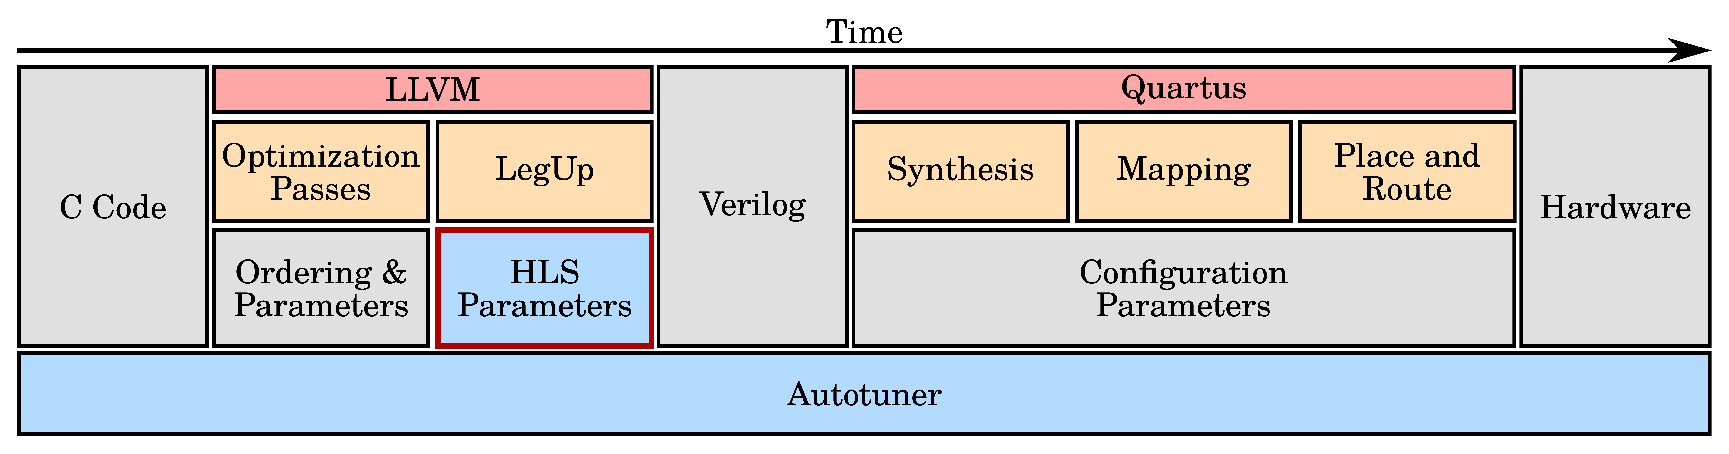
\includegraphics[width=.9\textwidth]{fpga-stack}
    \end{center}
    \end{block}
\end{frame}

\begin{frame}
    \frametitle{FPGAs: Autotuning for High-Level Synthesis}
    \begin{block}{Our \alert{autotuner setup}:}
    \begin{center}
        \includegraphics[width=.65\textwidth]{fpga_docker_tuner}
    \end{center}
    \end{block}
\end{frame}

\begin{frame}
    \frametitle{FPGAs: Autotuning for High-Level Synthesis}
    \begin{block}{Our HLS \alert{autotuning workflow}:}
    \begin{center}
        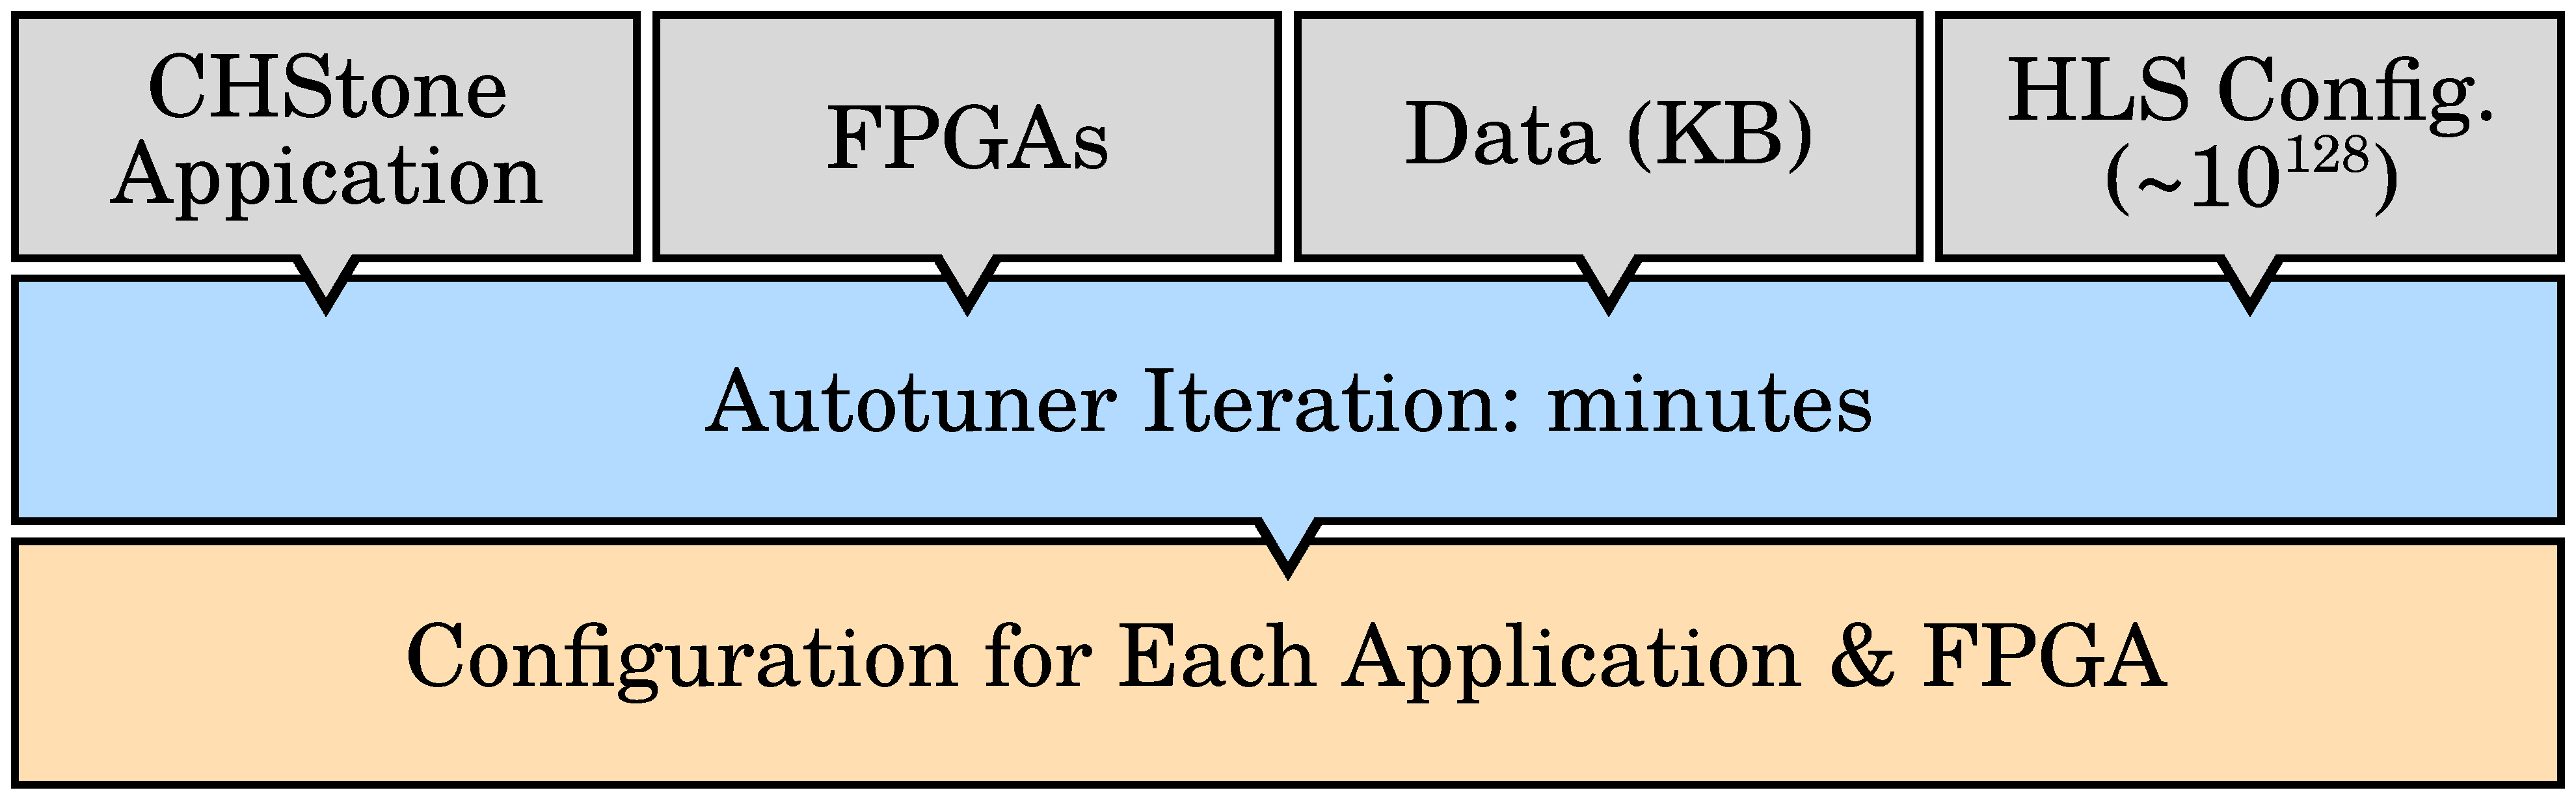
\includegraphics[width=.65\textwidth]{overview_fpgas_small}
    \end{center}
    \end{block}
\end{frame}

\section{Background}

\begin{frame}
    \frametitle{Related Work: Autotuning LLVM Passes for HLS}
        \alert{Huang, Qijing, \emph{et al.}}, \emph{"The effect of compiler
        optimizations on high-level synthesis-generated hardware." ACM
        Transactions on Reconfigurable Technology and Systems (2015)}:

    \begin{itemize}
        \item Optimizes \alert{parameters \& ordering} of a \alert{subset of
            LLVM passes}
        \item Uses \alert{LegUp} as an HLS tool
        \item Targets the \alert{Cyclone II} device family
        \item Uses the \alert{CHStone benchmark}
        \item Performs \alert{Exhaustive Search}
    \end{itemize}
\end{frame}

\begin{frame}
    \frametitle{Related Work: Autotuning Industry Designs for VTR}
        \alert{Xu \emph{et al.}}, \emph{"A Parallel Bandit-Based Approach
        for Autotuning FPGA Compilation." FPGA (2017)}:
        \begin{itemize}
            \item \alert{Does not optimize HLS}
            \item Optimizes \alert{parameters} of the
                \alert{Verilog-to-Routing} (\alert{VTR}) FPGA compilation tool
            \item Uses \alert{distributed OpenTuner instances}
        \end{itemize}
\end{frame}

\section{Experiments \& Results}

\begin{frame}
    \frametitle{High-Level Synthesis Benchmark}
    \begin{block}{C-based High-Level Synthesis \alert{benchmark}
        (\alert{CHStone}):}
        \begin{table}[htpb]
            \footnotesize
            \caption{Autotuned CHStone Applications}
            \centering
            \begin{tabular}{@{}p{0.1\columnwidth}p{0.5\columnwidth}@{}}
                \toprule
                Application & Short Description \\ \midrule
                blowfish & Symmetric-key block cypher \\
                aes & Advanced Encryption Algorithm (AES) \\
                adpcm & Adaptive Differential Pulse Code Modulation dec. and enc. \\
                sha & Secure Hash Algorithm (SHA) \\
                motion & Motion vector decoding from MPEG-2 \\
                mips & Simplified MIPS processor \\
                gsm & Predictive coding analysis of systems for mobile comms. \\
                dfsin & Sine function for double-precision floating-point numbers \\
                dfmul & Double-precision floating-point multiplication \\
                dfdiv & Double-precision floating-point division \\
                dfadd & Double-precision floating-point addition \\ \bottomrule
            \end{tabular}
        \end{table}
    \end{block}
\end{frame}

\begin{frame}
    \frametitle{Hardware Metrics}
    \begin{block}{\alert{Metric composition} problem:}
        \begin{itemize}
            \item \alert{8 hardware metrics} obtained from Quartus
            \item But the autotuner optimizes \alert{a single value}
        \end{itemize}
    \end{block}

    \begin{block}{Our \alert{solution} so far:}
        \begin{itemize}
            \item \alert{Normalize} metrics using initial values
            \item Optimize the \alert{normalized sum} of the 8 metrics
        \end{itemize}
    \end{block}
\end{frame}

\begin{frame}
    \frametitle{Hardware Metrics}
    \begin{block}{\alert{Normalized sum} of metrics:}
        \begin{align*} \label{eq:wnsm}
            \mathlarger{f(M, W)} = \frac{\mathlarger{\mathlarger{\mathlarger{\sum}}}\limits_{\substack{m_i \in M \\ w_i \in W}}{w_i\left(\dfrac{m_i}{m_{i}^{0}}\right)}}{\mathlarger{\mathlarger{\mathlarger{\sum}}}\limits_{w_i \in W}{w_i}}
        \end{align*}

        \begin{center}
            Where $M$ is the set of \alert{hardware metrics} and $W$ is the set
            of \alert{weights}
        \end{center}
    \end{block}
\end{frame}

\begin{frame}
    \frametitle{Weighted Optimization Scenarios}
    \begin{block}{An \alert{Optimization Scenario} consists of:}
        \begin{itemize}
            \item An \alert{optimization objective}: \alert{performance}, \alert{area}, $\dots$
            \item \alert{Weights} for \alert{hardware metrics}
        \end{itemize}
    \end{block}

    \begin{block}{Our scenarios:}
        \begin{itemize}
            \item 3 \alert{specific} scenarios \& 1 \alert{balanced} scenario
            \item Weights: \alert{powers of two} from 1: \alert{irrelevant} to
                8: \alert{high}
        \end{itemize}
    \end{block}
\end{frame}

\begin{frame}
    \frametitle{Weighted Optimization Scenarios}
        \begin{table}[htpb]
            \caption{\alert{Weights} for \alert{Optimization Scenarios} (\alert{High} $= 8$, \alert{Medium} $= 4$, \alert{Low} $= 2$)}
            \centering
            \begin{tabular}{@{}lcccc@{}}
                \toprule
                Metric & \textit{Area} & \textit{Perf. \& Lat} & \textit{Performance} & \textit{Balanced} \\ \midrule
                \textit{LUT} & \cellcolor[HTML]{9B94B6} High & \cellcolor[HTML]{DD9583} Low & \cellcolor[HTML]{DD9583} Low & \cellcolor[HTML]{E3DBB3} Medium \\
                \textit{Registers} & \cellcolor[HTML]{9B94B6} High & \cellcolor[HTML]{9B94B6} High & \cellcolor[HTML]{E3DBB3} Medium & \cellcolor[HTML]{E3DBB3} Medium \\
                \textit{BRAMs} & \cellcolor[HTML]{9B94B6} High & \cellcolor[HTML]{DD9583} Low & \cellcolor[HTML]{DD9583} Low & \cellcolor[HTML]{E3DBB3} Medium \\
                \textit{DSPs} & \cellcolor[HTML]{9B94B6} High & \cellcolor[HTML]{DD9583} Low & \cellcolor[HTML]{DD9583} Low & \cellcolor[HTML]{E3DBB3} Medium \\
                \textit{FMax} & \cellcolor[HTML]{DD9583} Low & \cellcolor[HTML]{9B94B6} High & \cellcolor[HTML]{9B94B6} High & \cellcolor[HTML]{E3DBB3} Medium \\
                \textit{Cycles} & \cellcolor[HTML]{DD9583} Low & \cellcolor[HTML]{9B94B6} High & \cellcolor[HTML]{DD9583} Low & \cellcolor[HTML]{E3DBB3} Medium \\ \bottomrule
            \end{tabular}
        \end{table}
\end{frame}

\begin{frame}
    \frametitle{Experiments}
    \begin{block}{Experiments}
        \begin{itemize}
            \item We performed 10 \alert{autotuning runs for each scenario}
            \item Each run took \alert{1.5 hours}
            \item We kept track of \alert{how each hardware metric changed over
                time}
            \item We used the \alert{Weighted Normalized Sum} (\alert{WNS}) as
                \alert{autotuning objective}
        \end{itemize}
    \end{block}
\end{frame}

\begin{frame}
    \frametitle{Results}
    \begin{block}{Presentation of results for each scenario:}
        \begin{itemize}
            \item \alert{Mean of the relative changes}, over 10 tuning runs
            \item For each \alert{hardware metric}, and for \alert{WNS}
            \item For each \alert{CHStone application}
            \item \alert{Bluer} is always better than \textcolor{red}{Redder}
        \end{itemize}
    \end{block}
\end{frame}

\begin{frame}
    \frametitle{Results: Comparing Default \& Random Starts}
    \begin{block}{Comparing \alert{Default} \& \alert{Random} starts:}
        \begin{itemize}
            \item A \alert{Default} start already provides a \alert{sensible
                optimization}
            \item A \alert{Random} start might favor the \alert{exploration of
                new, unintuitive solutions}
            \item In our case, the \alert{Default} start was provided to the
                \alert{StratixV FPGA} by \alert{LegUp}
        \end{itemize}
    \end{block}
\end{frame}

\begin{frame}
    \frametitle{Results: Comparing Default \& Random Starts}
        \begin{figure}[htpb]
            \centering
            \includegraphics[width=0.8\columnwidth]{heatmap_comp_stratixV}
            \caption{Comparison of the absolute values for Random and Default
            starting points in the Balanced scenario}
        \end{figure}
\end{frame}

\begin{frame}
    \frametitle{Results: Comparing Default \& Random Starts}
    \begin{block}{Comparing \alert{Default} \& \alert{Random} starts:}
        \begin{itemize}
            \item The \alert{Default} start achieves \alert{better absolute
                values} than the \alert{Random} start, on most cases
            \item The next results were obtained using the \alert{Default}
                start
        \end{itemize}
    \end{block}
\end{frame}

\begin{frame}
    \frametitle{Results: the Balanced Scenario}
    \begin{columns}[T,onlytextwidth]
        \column{0.2\textwidth}
        \begin{table}[htpb]
            \scriptsize
            \centering
            \begin{tabular}{@{}lcccc@{}}
                \toprule
                Metric & \textit{Balanced} \\ \midrule
                \textit{LUT} & \cellcolor[HTML]{E3DBB3} Medium \\
                \text   it{Registers} & \cellcolor[HTML]{E3DBB3} Medium \\
                \textit{BRAMs} & \cellcolor[HTML]{E3DBB3} Medium \\
                \textit{DSPs} & \cellcolor[HTML]{E3DBB3} Medium \\
                \textit{FMax} & \cellcolor[HTML]{E3DBB3} Medium \\
                \textit{Cycles} & \cellcolor[HTML]{E3DBB3} Medium \\ \bottomrule
            \end{tabular}
        \end{table}

        \column{0.8\textwidth}
        \begin{figure}[htpb]
            \centering
            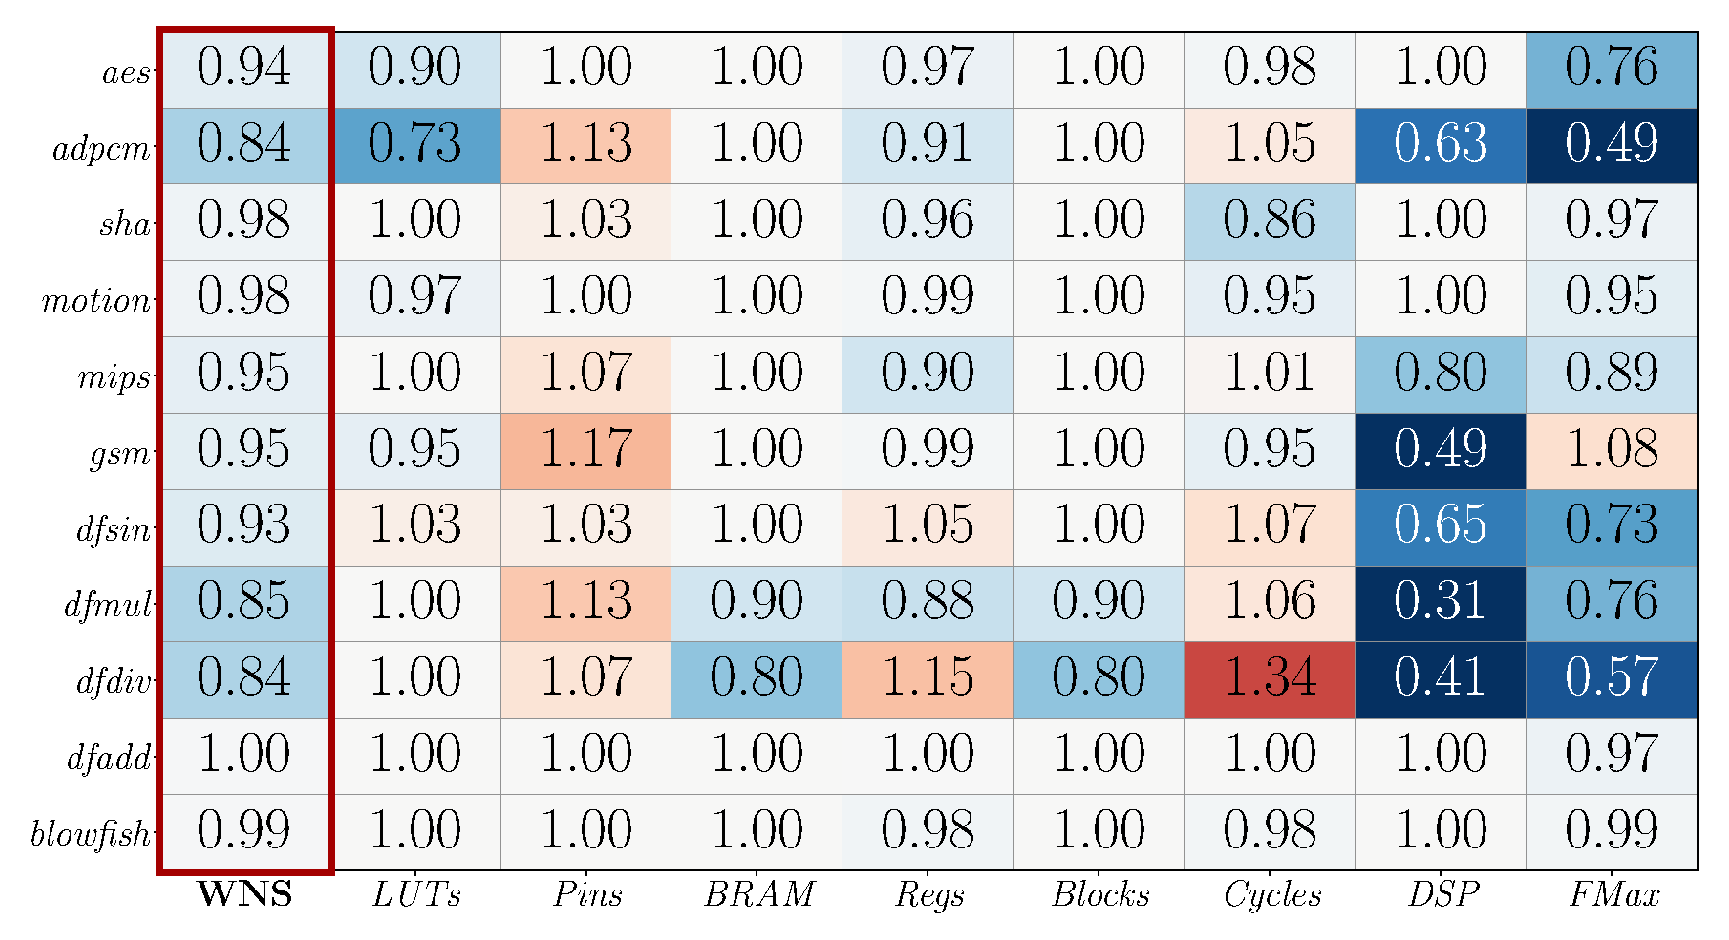
\includegraphics[width=0.8\columnwidth]{heatmap_default_stratixV}
            \caption{Relative improvement for all metrics in the \textit{Balanced}
            scenario}
        \end{figure}
    \end{columns}
\end{frame}

\begin{frame}
    \frametitle{Results: the Area Scenario}
    \begin{columns}[T,onlytextwidth]
        \column{0.2\textwidth}
        \begin{table}[htpb]
            \scriptsize
            \centering
            \begin{tabular}{@{}lcccc@{}}
                \toprule
                Metric & \textit{Area} \\ \midrule
                \textit{LUT} & \cellcolor[HTML]{9B94B6} High \\
                \textit{Registers} & \cellcolor[HTML]{9B94B6} High \\
                \textit{BRAMs} & \cellcolor[HTML]{9B94B6} High \\
                \textit{DSPs} & \cellcolor[HTML]{9B94B6} High \\
                \textit{FMax} & \cellcolor[HTML]{DD9583} Low \\
                \textit{Cycles} & \cellcolor[HTML]{DD9583} Low \\ \bottomrule
            \end{tabular}
        \end{table}

        \column{0.8\textwidth}
        \begin{figure}[htpb]
            \centering
            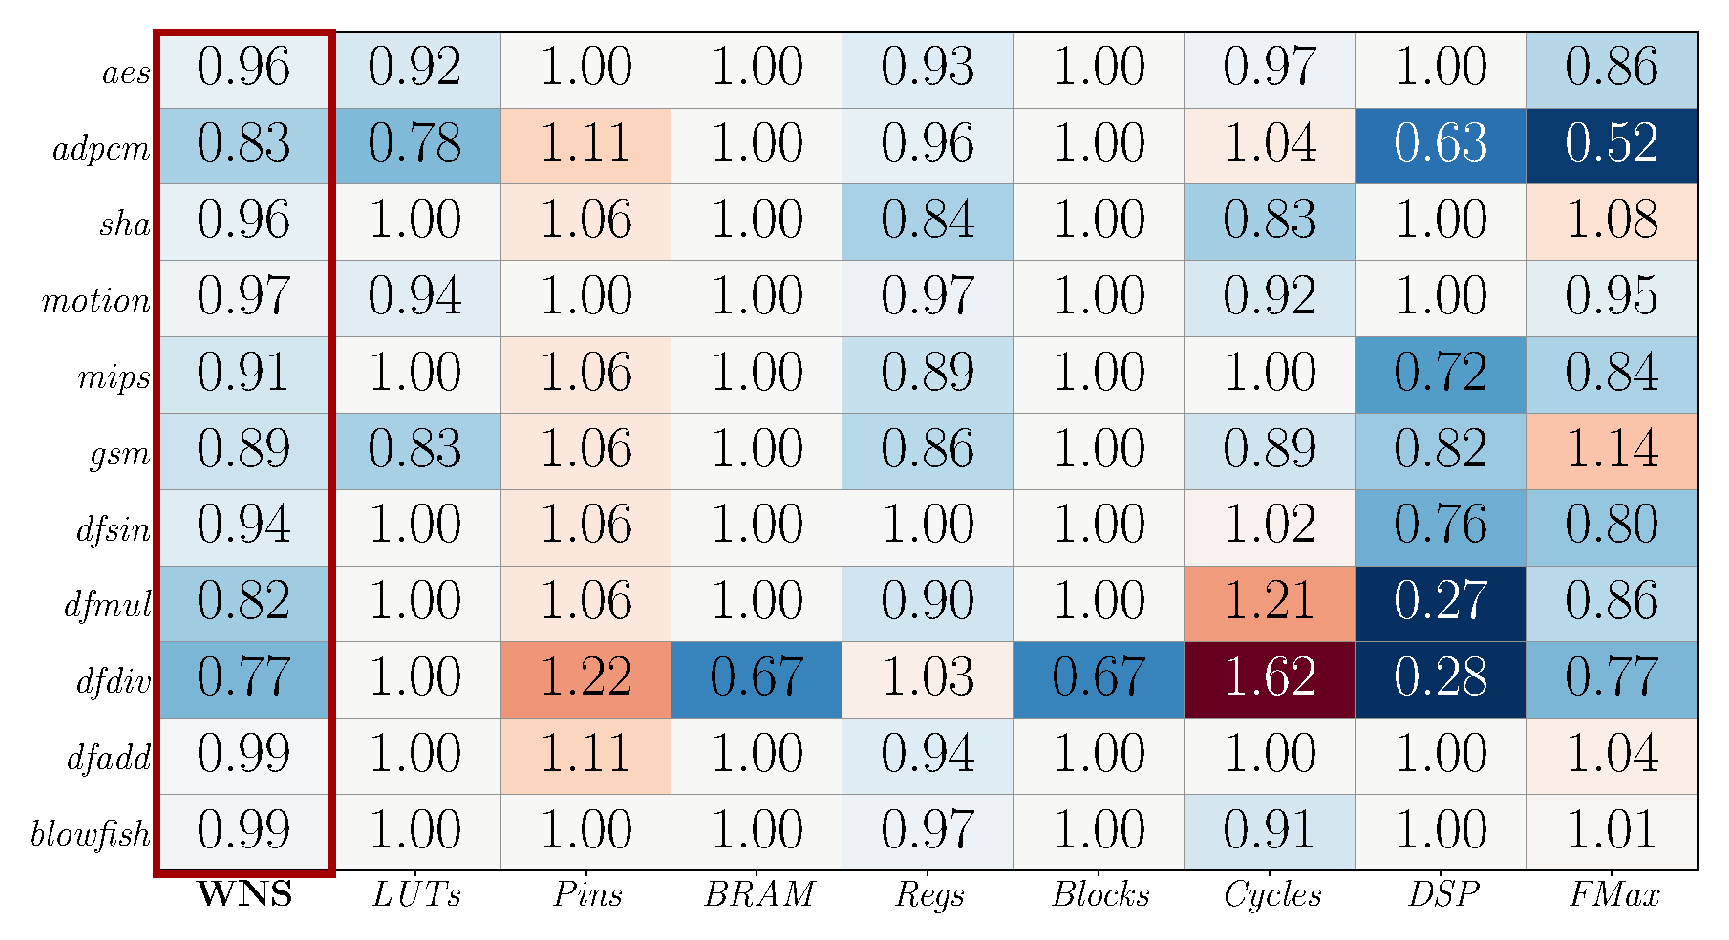
\includegraphics[width=0.8\columnwidth]{heatmap_default_stratixV_area}
            \caption{Relative improvement for all metrics in the \textit{Area}
            scenario}
        \end{figure}
    \end{columns}
\end{frame}

\begin{frame}
    \frametitle{Results: the Performance Scenario}
    \begin{columns}[T,onlytextwidth]
        \column{0.2\textwidth}
        \begin{table}[htpb]
            \scriptsize
            \centering
            \begin{tabular}{@{}lcccc@{}}
                \toprule
                Metric & \textit{Performance} \\ \midrule
                \textit{LUT} & \cellcolor[HTML]{DD9583} Low \\
                \textit{Registers} & \cellcolor[HTML]{E3DBB3} Medium \\
                \textit{BRAMs} & \cellcolor[HTML]{DD9583} Low \\
                \textit{DSPs} & \cellcolor[HTML]{DD9583} Low \\
                \textit{FMax} & \cellcolor[HTML]{9B94B6} High \\
                \textit{Cycles} & \cellcolor[HTML]{DD9583} Low \\ \bottomrule
            \end{tabular}
        \end{table}

        \column{0.8\textwidth}
        \begin{figure}[htpb]
            \centering
            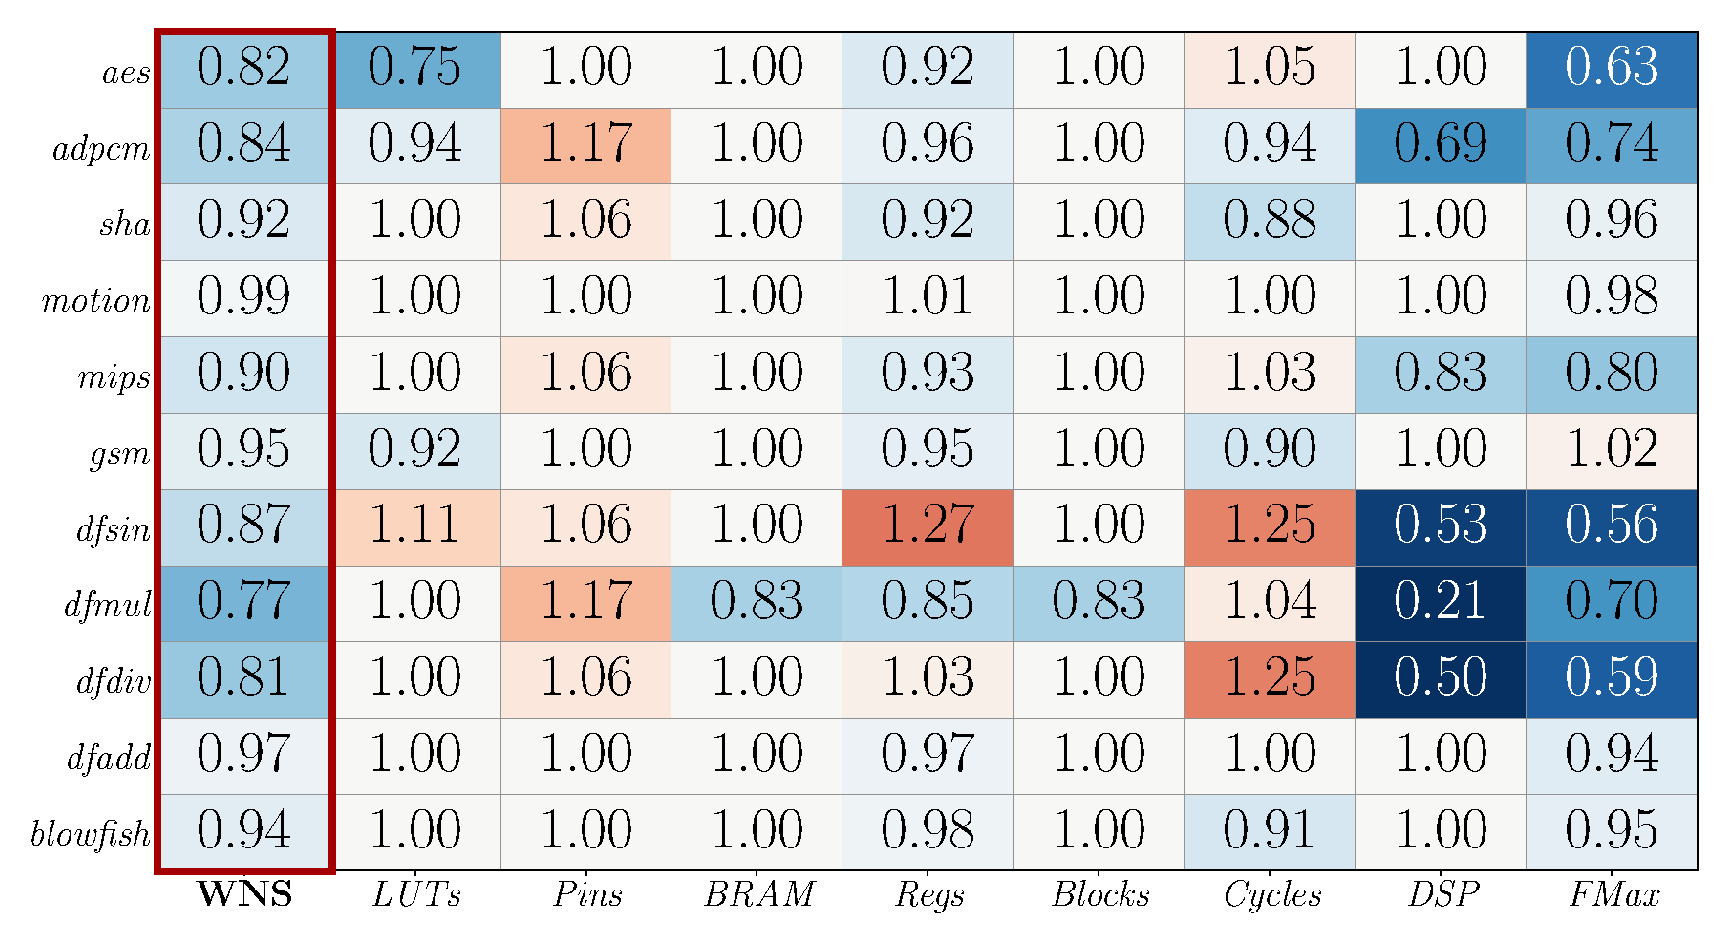
\includegraphics[width=0.8\columnwidth]{heatmap_default_stratixV_perf}
            \caption{Relative improvement for all metrics in the
            \textit{Performance} scenario}
        \end{figure}
    \end{columns}
\end{frame}

\begin{frame}
    \frametitle{Results: the Performance \& Latency Scenario}
    \begin{columns}[T,onlytextwidth]
        \column{0.2\textwidth}
        \begin{table}[htpb]
            \scriptsize
            \centering
            \begin{tabular}{@{}lcccc@{}}
                \toprule
                Metric & \textit{Perf. \& Lat} \\ \midrule
                \textit{LUT} & \cellcolor[HTML]{DD9583} Low \\
                \textit{Registers} & \cellcolor[HTML]{9B94B6} High \\
                \textit{BRAMs} & \cellcolor[HTML]{DD9583} Low \\
                \textit{DSPs} & \cellcolor[HTML]{DD9583} Low \\
                \textit{FMax} & \cellcolor[HTML]{9B94B6} High \\
                \textit{Cycles} & \cellcolor[HTML]{9B94B6} High \\ \bottomrule
            \end{tabular}
        \end{table}

        \column{0.8\textwidth}
        \begin{figure}[htpb]
            \centering
            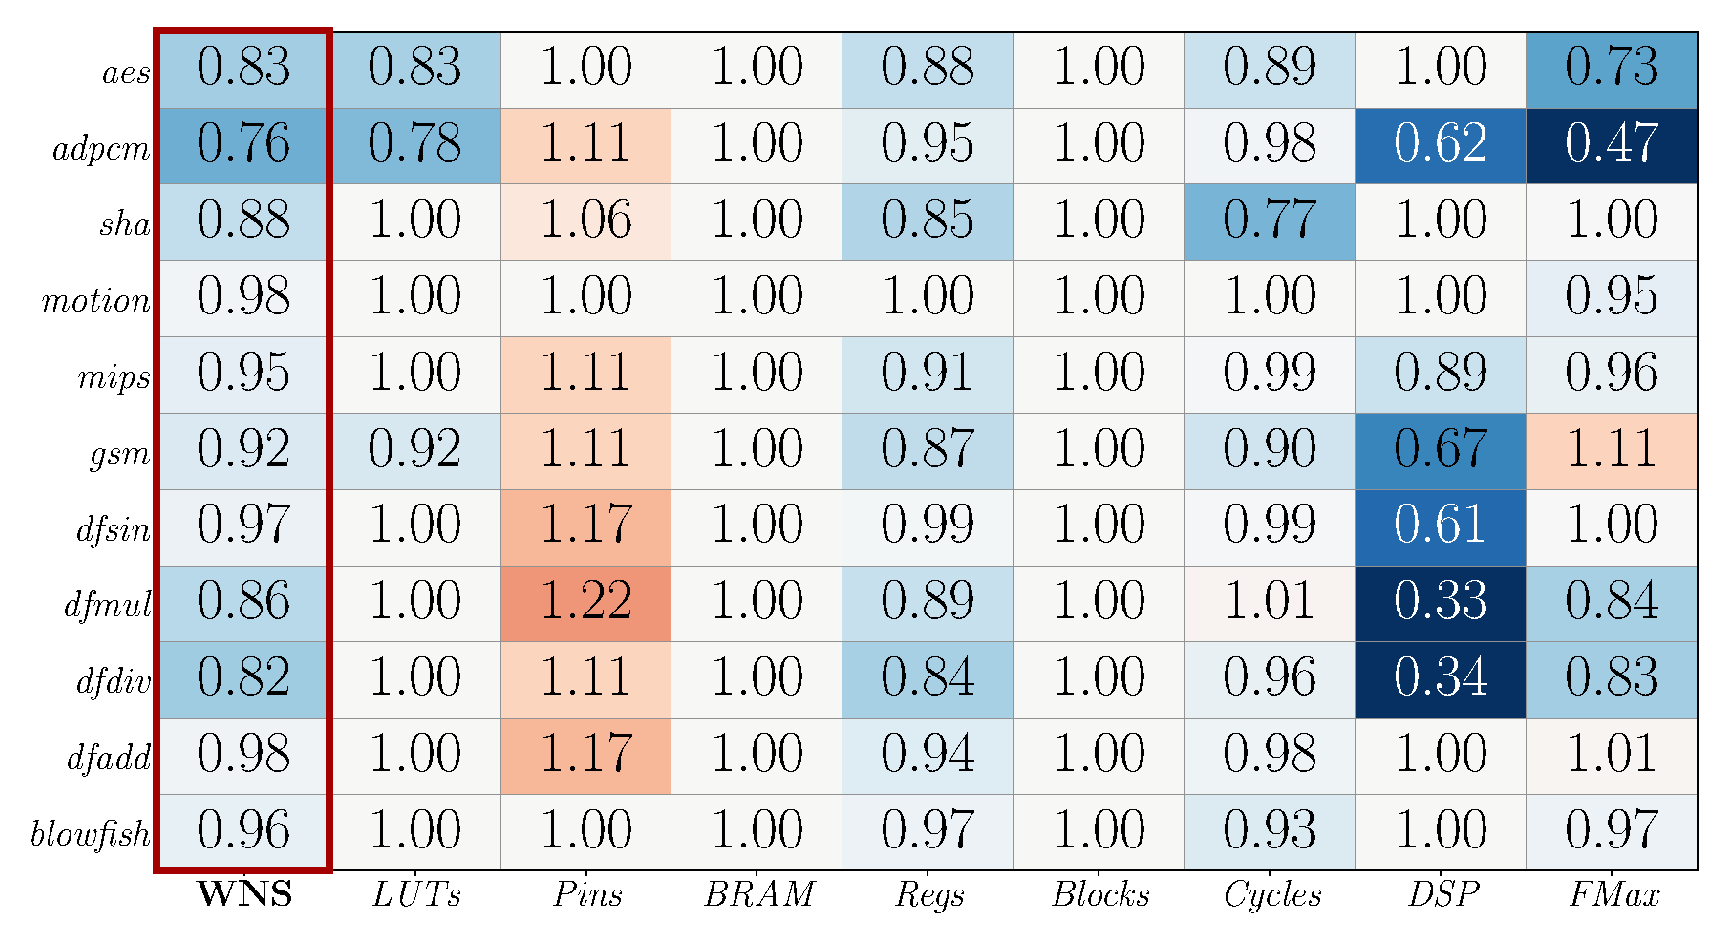
\includegraphics[width=0.8\columnwidth]{heatmap_default_stratixV_perflat}
            \caption{Relative improvement for all metrics in the
            \textit{Performance \& Latency} scenario}
        \end{figure}
    \end{columns}
\end{frame}

\begin{frame}
    \frametitle{Results: Comparing the Weighted Normalized Sum (WNS)}
    \begin{figure}[htpb]
        \centering
        \includegraphics[width=0.8\columnwidth]{heatmap_wns_comparison}
        \caption{Relative improvement for \textbf{WNS} in all scenarios}
    \end{figure}
\end{frame}

\section{Conclusion}

\begin{frame}
    \frametitle{Results: Conclusion}
    \begin{block}{In all scenarios:}
        \begin{itemize}
            \item Heavily weighted metrics \alert{improved the most}
            \item Lightly weighted or irrelevant metrics \alert{did not worsen
                greatly}
        \end{itemize}
    \end{block}

    \begin{block}{Autotuning starting point:}
        \begin{itemize}
            \item A random start \alert{might achieve more relative
                improvement}
            \item But a sensible start \alert{achieves better absolute values}
        \end{itemize}
    \end{block}
\end{frame}

\begin{frame}
    \frametitle{Limitations of this Work}
    \begin{block}{Issues with the \alert{Weighted Normalized Sum}:}
        \begin{itemize}
            \item The WNS is a \alert{very naive metric combination strategy}
            \item The \alert{multi-objective optimization} domain provides
                \alert{better approaches}
        \end{itemize}
    \end{block}
\end{frame}

\begin{frame}
    \frametitle{Future Work}
    \begin{block}{\alert{Bigger designs}:}
        \begin{itemize}
            \item CHStone \alert{designs are very simple}
            \item We will use our autotuning approach for \alert{bigger FPGA
                designs}
        \end{itemize}
    \end{block}

    \begin{block}{\alert{Compiler configuration}:}
        \begin{itemize}
            \item HLS usually includes a C/C++ \alert{compiler step}
            \item We will include \alert{compiler parameters or passes} in our
                autotuner
        \end{itemize}
    \end{block}

    \begin{block}{\alert{Other HLS tools}:}
        \begin{itemize}
            \item Other HLS tools provide \alert{different search spaces}
            \item We will use our autotuning approach for more
                \alert{proprietary and open HLS tools}
            \item We want to use cost models that \alert{predict hardware
                metrics before synthesis}
        \end{itemize}
    \end{block}
\end{frame}

\begin{frame}
    \frametitle{Conclusion}
    \begin{block}{Autotuning HLS for FPGAs:}
        \begin{itemize}
            \item Designers can \alert{select optimization objectives using
                weights}
            \item Good \alert{WNS improvements} after \alert{1.5 hours} of
                autotuning
            \item Improvements for targeted metrics \alert{without worsening
                other metrics}
            \item A \alert{sensible starting point} impacts autotuning results
                positively
        \end{itemize}
    \end{block}
\end{frame}

\maketitle

\end{document}
